\documentclass[12pt,a4paper,twoside,english]{book}

\usepackage{Formato}
\usepackage{sectsty}
\title{Tesis 9 Anexos }
\author{Aaron Sújar}

\begin{document}
\frontmatter

\thispagestyle{empty}
\chapter*{Acronyms}

\begin{acronym}

\acro{B-rep}{representación superficial}
\acro{Bangor}{Bangor University}
\acro{DQS}{dual quaternion skinning}
\acro{CAD}{diseño asistido por computador}
\acro{COR}{centros de rotación}
\acro{Courseware}{aplicación de entrenamiento}
\acro{DICOM}{Imagen y Comunicación Digital en Medicina}
\acro{DOF}{grados de libertad}
\acro{E/S}{Entrada/Salida}
\acro{EASA}{Agencia Europea de Seguridad Aérea}
\acro{FEM}{método de elementos finitos}
\acro{FORTH}{Foundation for Research and Technology - Hellas}
\acro{CGAL}{Computational Geometry Algorithms Library}
\acro{GLSL}{OpenGL Shading Language}
\acro{GMRV}{Grupo de Modelado y Realidad Virtual}
\acro{GPL}{GNU General Public License}
\acro{GPU}{unidad de procesamiento gráfico}
\acro{ITGVPH}{Integrated Toolkit for Generation of VPH Models}
\acro{INRIA}{Institut National de Recherche en Informatique et en Automatique}
\acro{IRM}{imagen por resonancia magnética}
\acro{IU}{interfaz de usuario}
\acro{joints}{articulaciones virtuales}
\acro{kvp}{tensión de pico}
\acro{kV}{kV}{kilovoltio}
\acro{keV}{keV}{kiloelectronvoltio}
\acro{LGPL}{GNU Lesser General Public License}
\acro{LBS}{linear blending skinning}
\acro{mAs}{mAs}{miliamperio por segundo}
\acro{MoCap}{captura de movimientos}
\acro{RA}{anestesia regional}
\acro{RAAs}{Regional Anaesthesia Assistant}
\acro{RAM}{Random Access Memory}
\acro{RASim}{Regional Anaesthesia Simulator}
\acro{RASimAs}{Regional Anaesthesia Simulator and Assistant}
\acro{RDT}{triangulación restringida de delaunay}
\acro{RV}{realidad virtual}
\acro{RWTH}{RWTH Aachen University}
\acro{SBS}{Spherical Blend Skinning}
\acro{SINTEF}{Stiftelsen for industriell og teknisk forskning}
\acro{SG}{Sensegraphics}
\acro{SOFA}{Simulation Open Framework Architecture}
\acro{TASMIP}{TASMIP}{tungsten anode spectral model using interpolating polynomials}
\acro{TC}{tomografía axial computarizada}
\acro{TPTVPH}{Toolkit for Pose Transforms of VPH Models}
\acro{tracker}{dispositivo de seguimiento}
\acro{tabla hash}{Spatial Hash Table}
\acro{UKA-IMI}{Department of Medical Informatics: Uniklinik RWTH Aachen}
\acro{URJC}{Universidad Rey Juan Carlos}
\acro{US}{ultrasonidos} 
\acro{ViSTA}{Virtual Reality Toolkit}
\acro{VPH}{pacientes virtuales}
\acro{VTU}{formato de Visualization Toolkit}
\acro{WP}{paquetes de trabajos}
\acro{X3D}{formato Extensible 3D}
\acro{XML}{Extensible Markup Language}
\acro{ZPD}{zona de desarrollo próximo}


\end{acronym}


\pagenumbering{roman}

%\include{ack}

%\appendix
\chapter*{Apéndices}
\tableofcontents
\mainmatter
\setboolean{@twoside}{false}




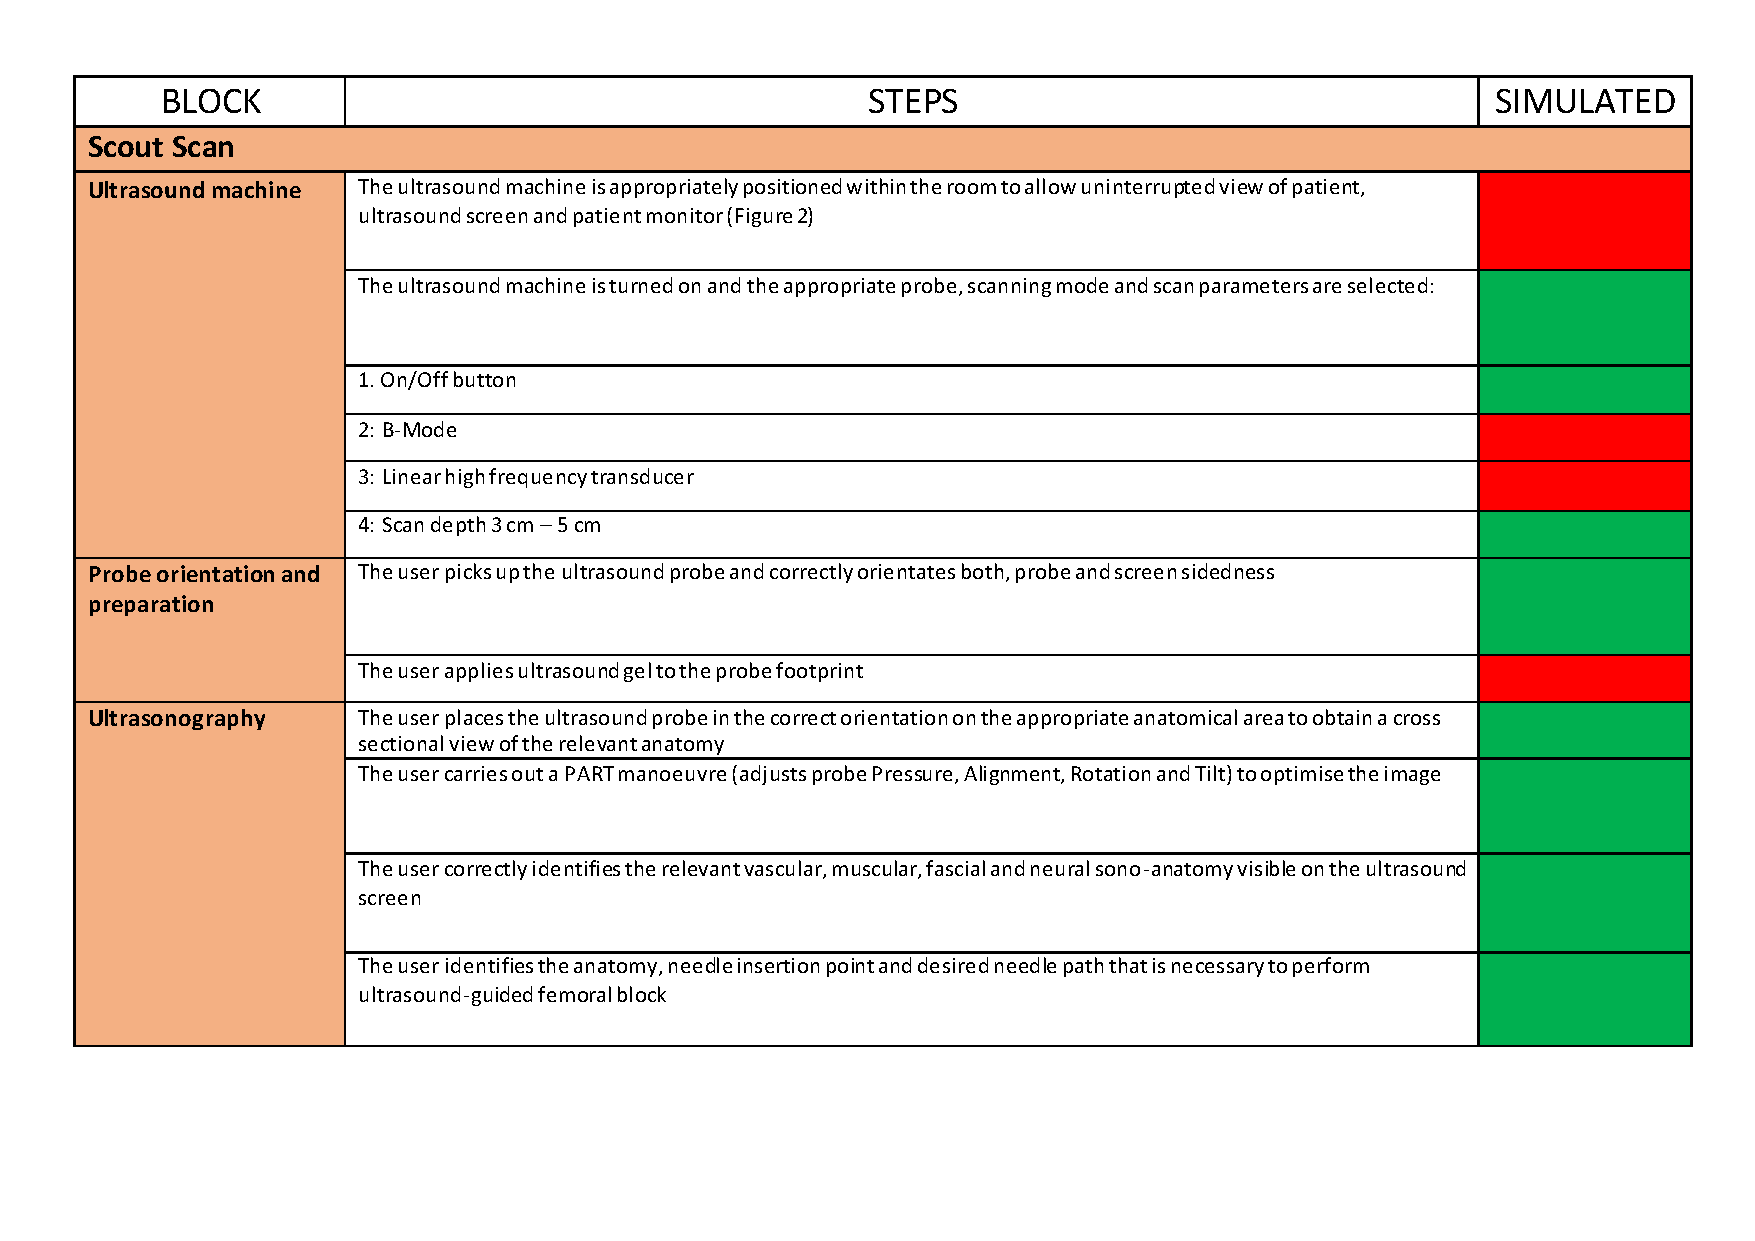
\includepdf[pages=1,landscape,scale=0.8,
pagecommand={\section{Descripción del procedimiento de \ac{RA}}
\label{anexo:RA}},linktodoc=true]{PDFs/RA}
\includepdf[pages=2-,landscape,scale=0.85,pagecommand={},linktodoc=true]{PDFs/RA}


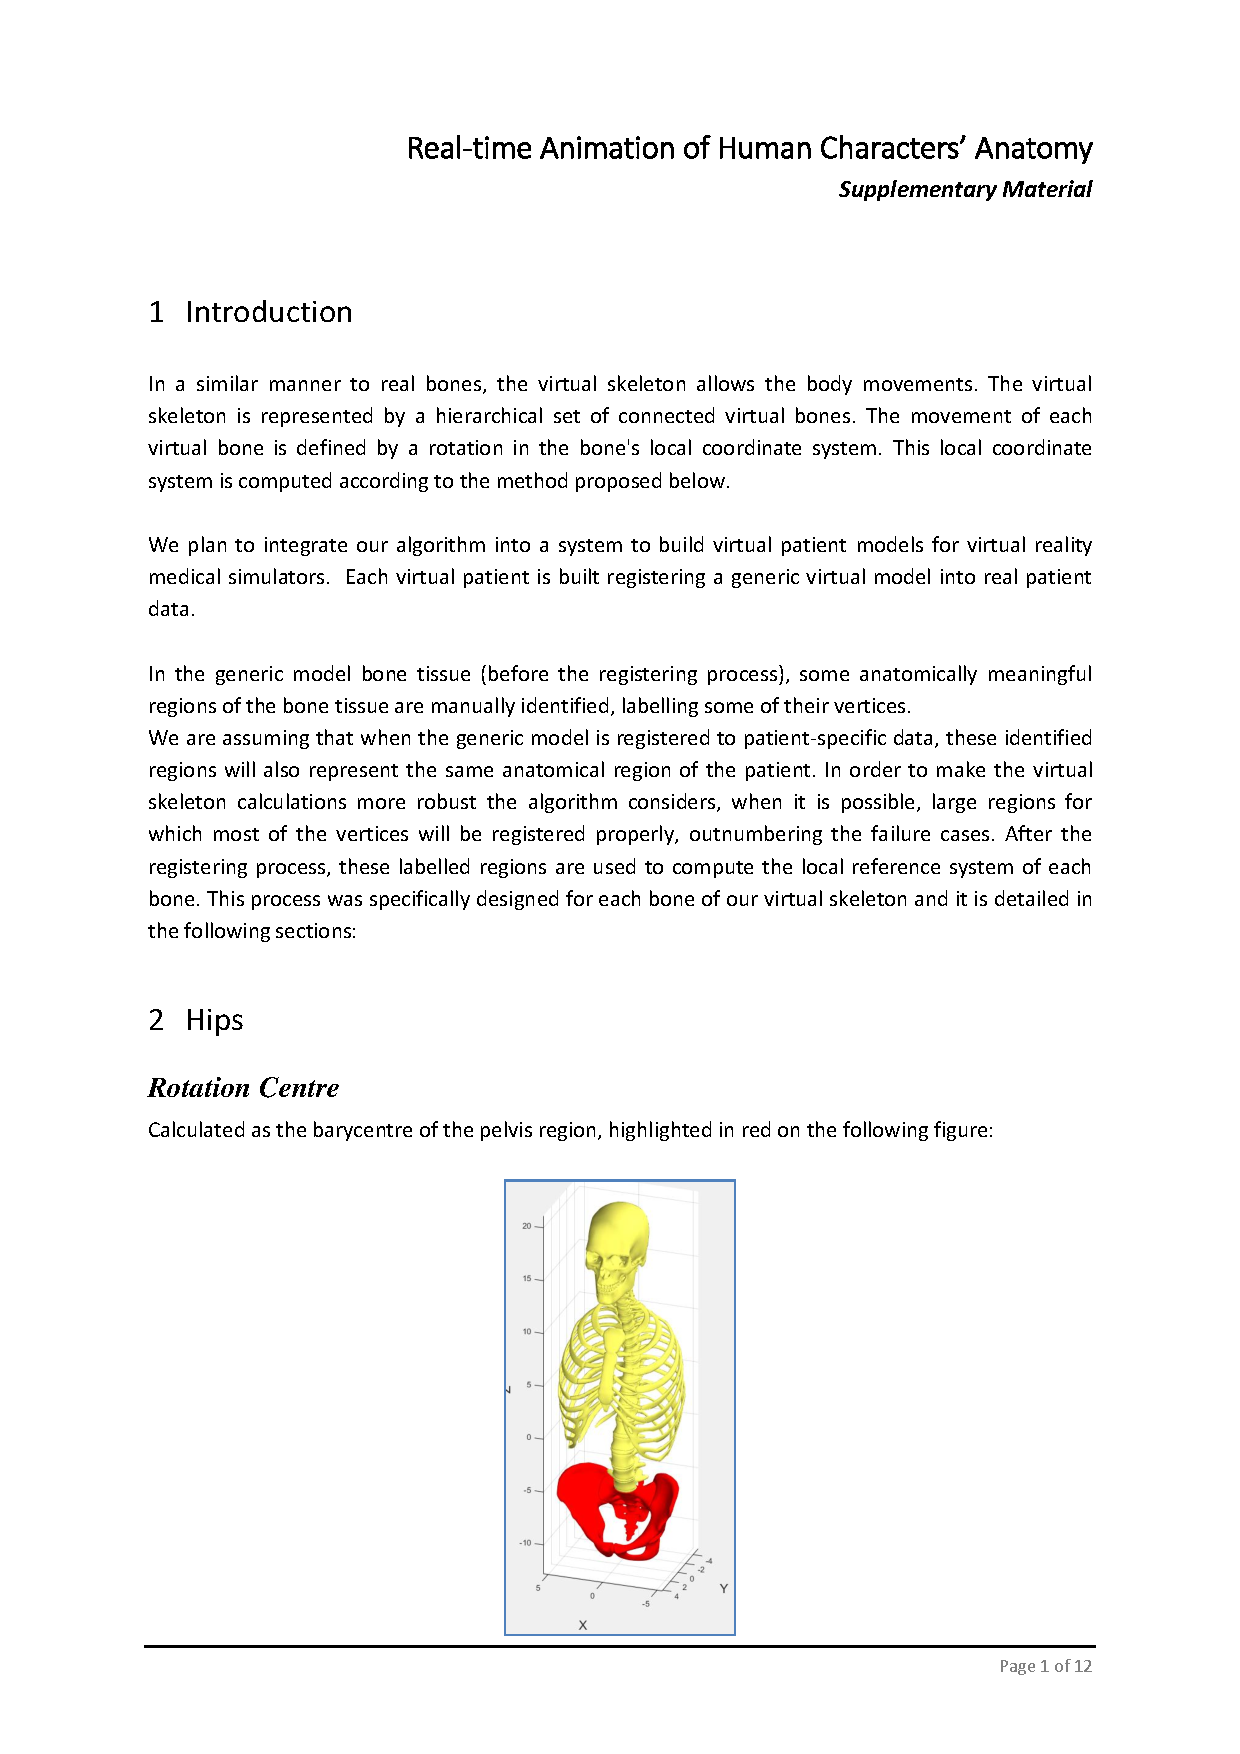
\includepdf[pages=1,scale=0.8,
pagecommand={\section{Rigging para cada hueso}
\label{anexo:rigging}},linktodoc=true]{PDFs/Supplementary}
\includepdf[pages=2-,scale=0.88,pagecommand={},linktodoc=true]{PDFs/Supplementary}

\section{Parámetros del refinamiento utilizando \ac{RDT}}
\label{anexo:criterios}


\begin{figure}[h]
   \centering
    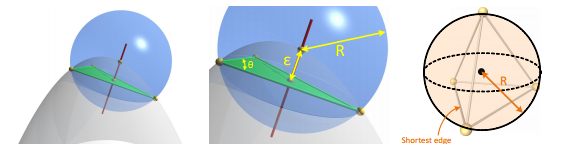
\includegraphics[width=0.8\textwidth]{IMG/rdt.png}
     \caption{Triangulación Restringida de Delaunay (\acs{RDT}). A la izquierda, faceta superficial con esfera de \emph{Delunay}. En el centro, detalle de los criterios utilizados para el refinamiento. A la derecha, \emph{circunsfera} asociada a un tetraedro.}
\label{fig:rdt}
\end{figure}


La \ac{RDT} es un algoritmo iterativo que genera una malla de tetraedros atendiendo a una serie de criterios de tamaño y forma. En primer lugar se definen una serie de elementos geométricos sobre los cuales se comprueban las restricciones (figura \ref{fig:rdt}).

\begin{itemize}
    \item Faceta superficial: Faceta de un tetraedro que aproxima la superficie del dominio
    \item Esfera de \emph{Delaunay}: Esfera de radio mínimo con centro en la superficie del dominio y que contiene a la faceta superficial
    \item \emph{Circumsfera} (asociada al tetraedro): Esfera de radio mínimo que contiene los cuatro vértices de un tetraedro
\end{itemize}




Las restricciones sobre las facetas superficiales son las siguientes:
\begin{itemize}
    \item  Tamaño: Radio máximo de la esfera de \emph{Delaunay}
    \item Forma: Límite inferior para los ángulos de la faceta superficial
    \item Aproximación: Distancia máxima entre la faceta superficial y el centro de la esfera de \emph{Delaunay}

\end{itemize}

Las restricciones sobre los tetraedros son las siguientes:
\begin{itemize}
    \item Tamaño: Radio máximo de la \emph{circumsfera}
    \item Forma: Relación máxima entre el \emph{circumradio} y la arista mas corta del tetraedro
\end{itemize}



Gracias a estos criterios, es posible controlar tanto la aproximación de la malla de tetraedros a la superficie como el tamaño general de tetraedros y triángulos, consiguiendo así reducir el número de tetraedros en las zonas donde no hacen falta y aumentando la resolución allí donde se requiera una mejor aproximación.

%\label{anexo:RA}

% \section{Cuestionario Comparación COR vs FEM }
% \includepdf[pages=-,pagecommand={},frame,nup=3x3,scale=0.75]{PDFs/Real-timeQ}
% \label{anexo:cuestionario1}

%\chapter{Cuestionario Comparación COR vs FEM }

\includepdf[pages=1,scale=0.8,
pagecommand={\section{Cuestionario Comparación COR vs FEM}
\label{anexo:cuestionario2}},linktodoc=true]{PDFs/DeformationQ}
\includepdf[pages=2-,scale=0.9,nup=2x2,pagecommand={},linktodoc=true]{PDFs/DeformationQ}

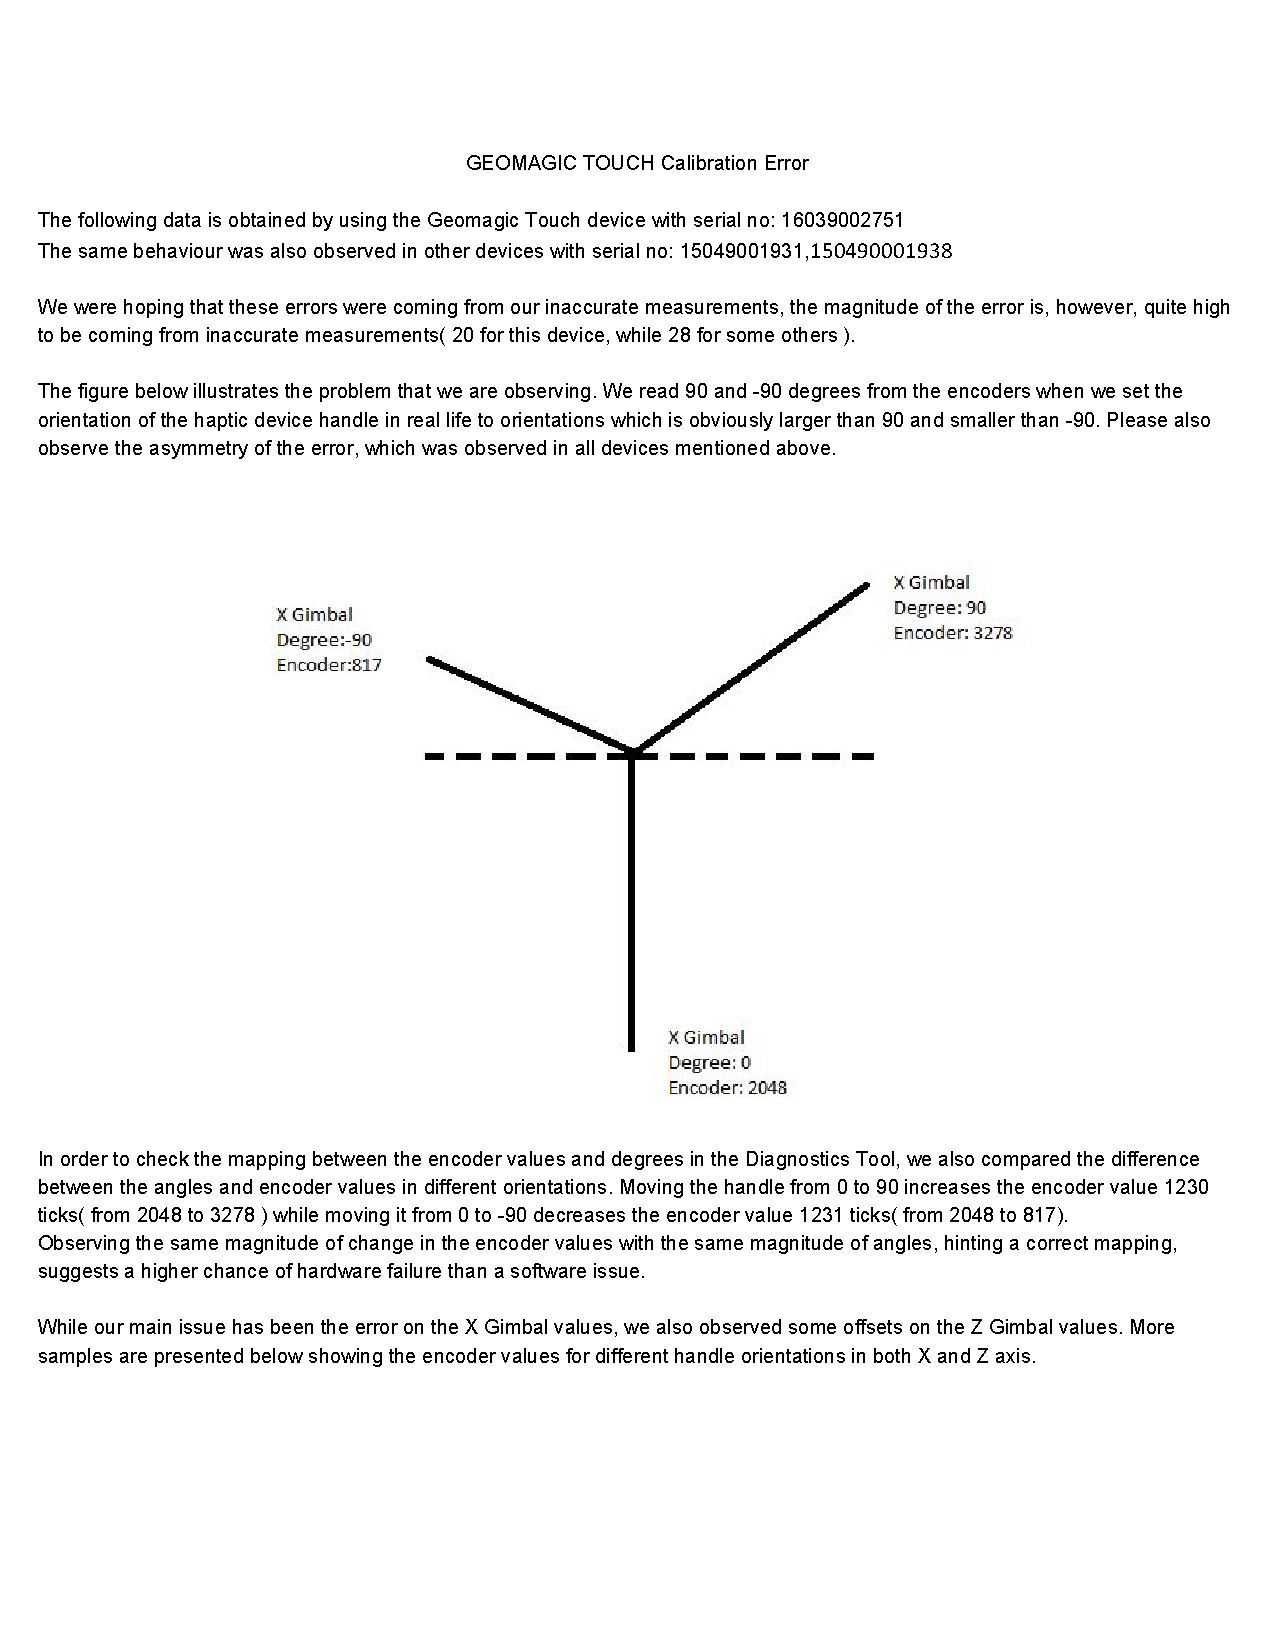
\includepdf[pages=1,scale=0.8,
pagecommand={\section{Carta describiendo los errores econtrados en los dispositivos Touch}
\label{anexo:geomagic}},linktodoc=true]{PDFs/GeoMagic}
\includepdf[pages=2-,scale=1,pagecommand={},linktodoc=true]{PDFs/GeoMagic}

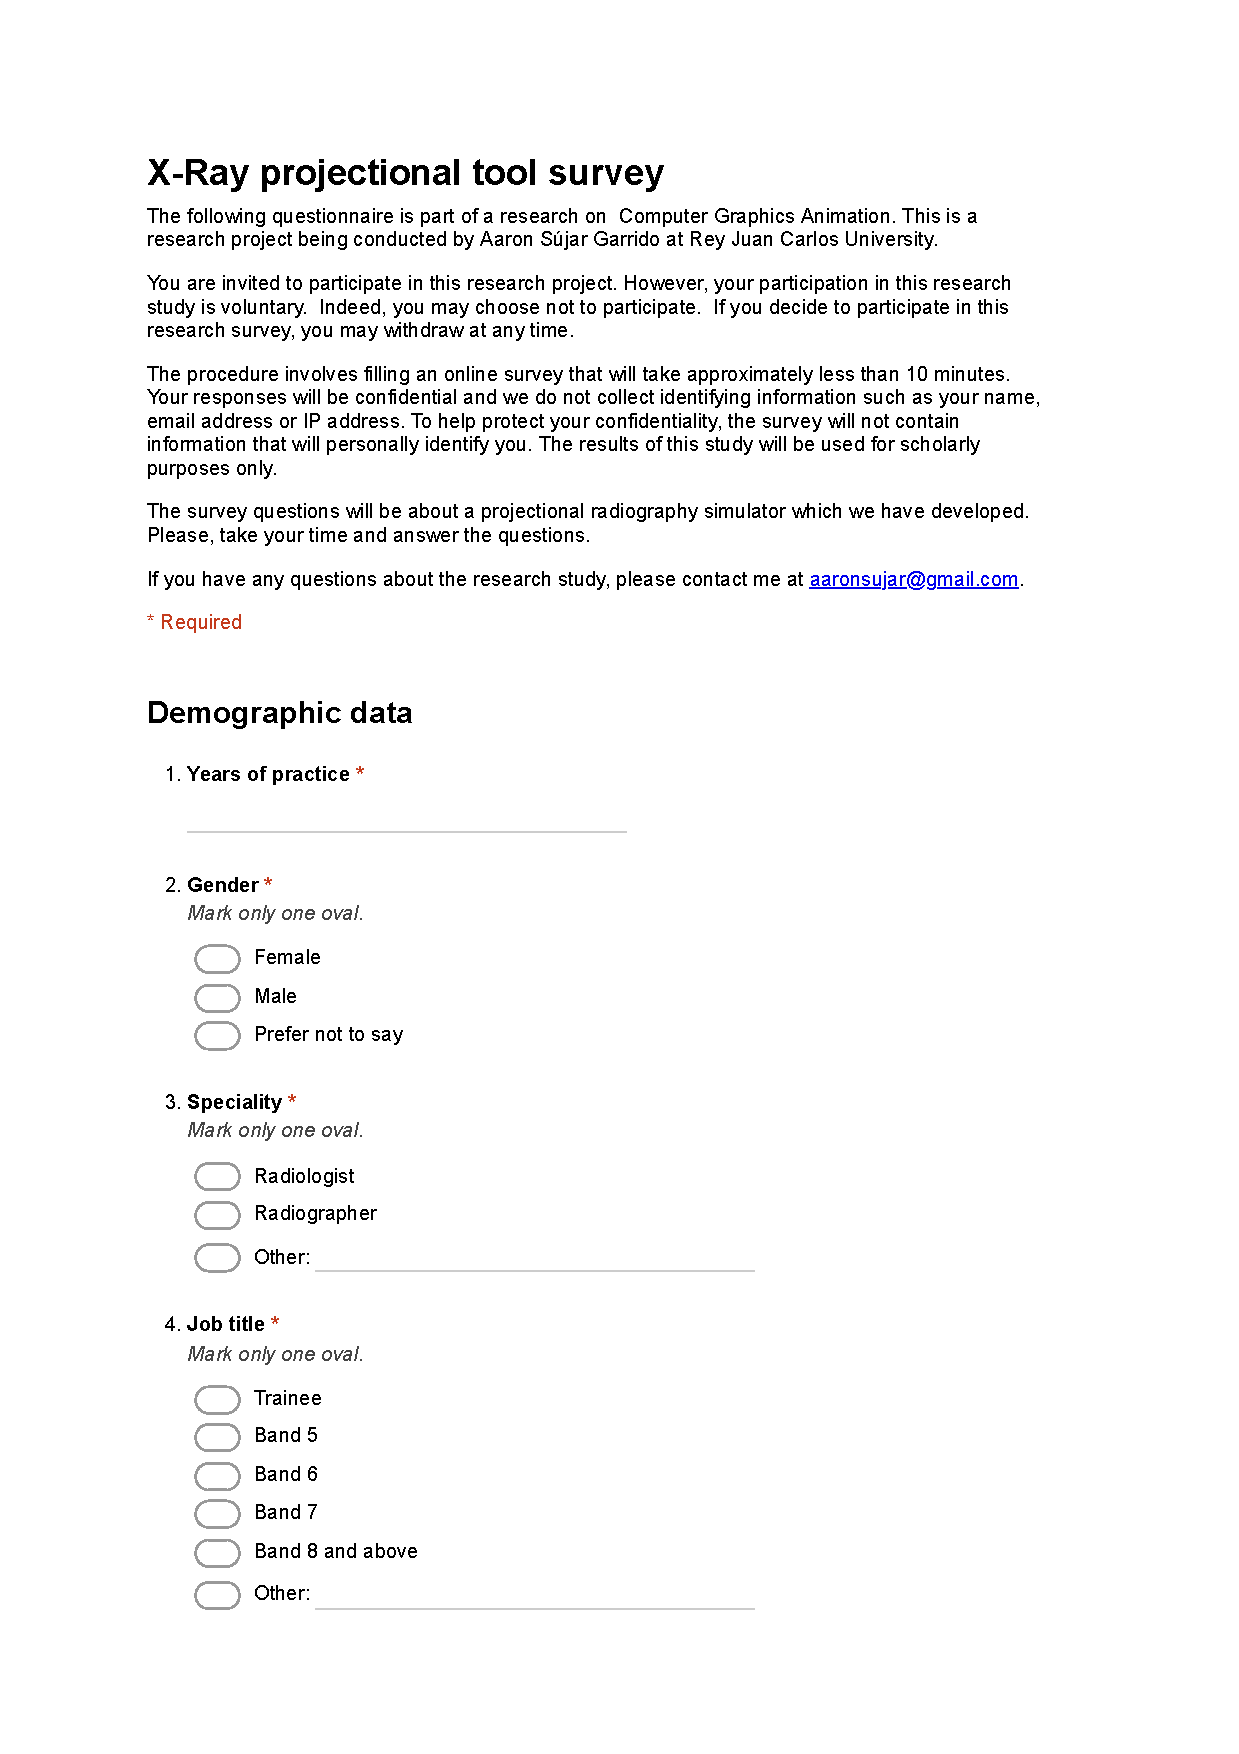
\includepdf[pages=1,scale=0.8,
pagecommand={\section{Cuestionario de validez aparente y de contenido}
\label{anexo:cuestionarioxray}},linktodoc=true]{PDFs/xraysurvey}
\includepdf[pages=2-,scale=0.9,pagecommand={},linktodoc=true]{PDFs/xraysurvey}




\includepdf[pages=1,scale=0.8,
pagecommand={\section{An Interactive Algorithm for Virtual Patient Positioning}
\label{anexo:ceig}},linktodoc=true]{PDFs/ceig}
\includepdf[pages=2-,scale=1,pagecommand={},linktodoc=true]{PDFs/ceig}


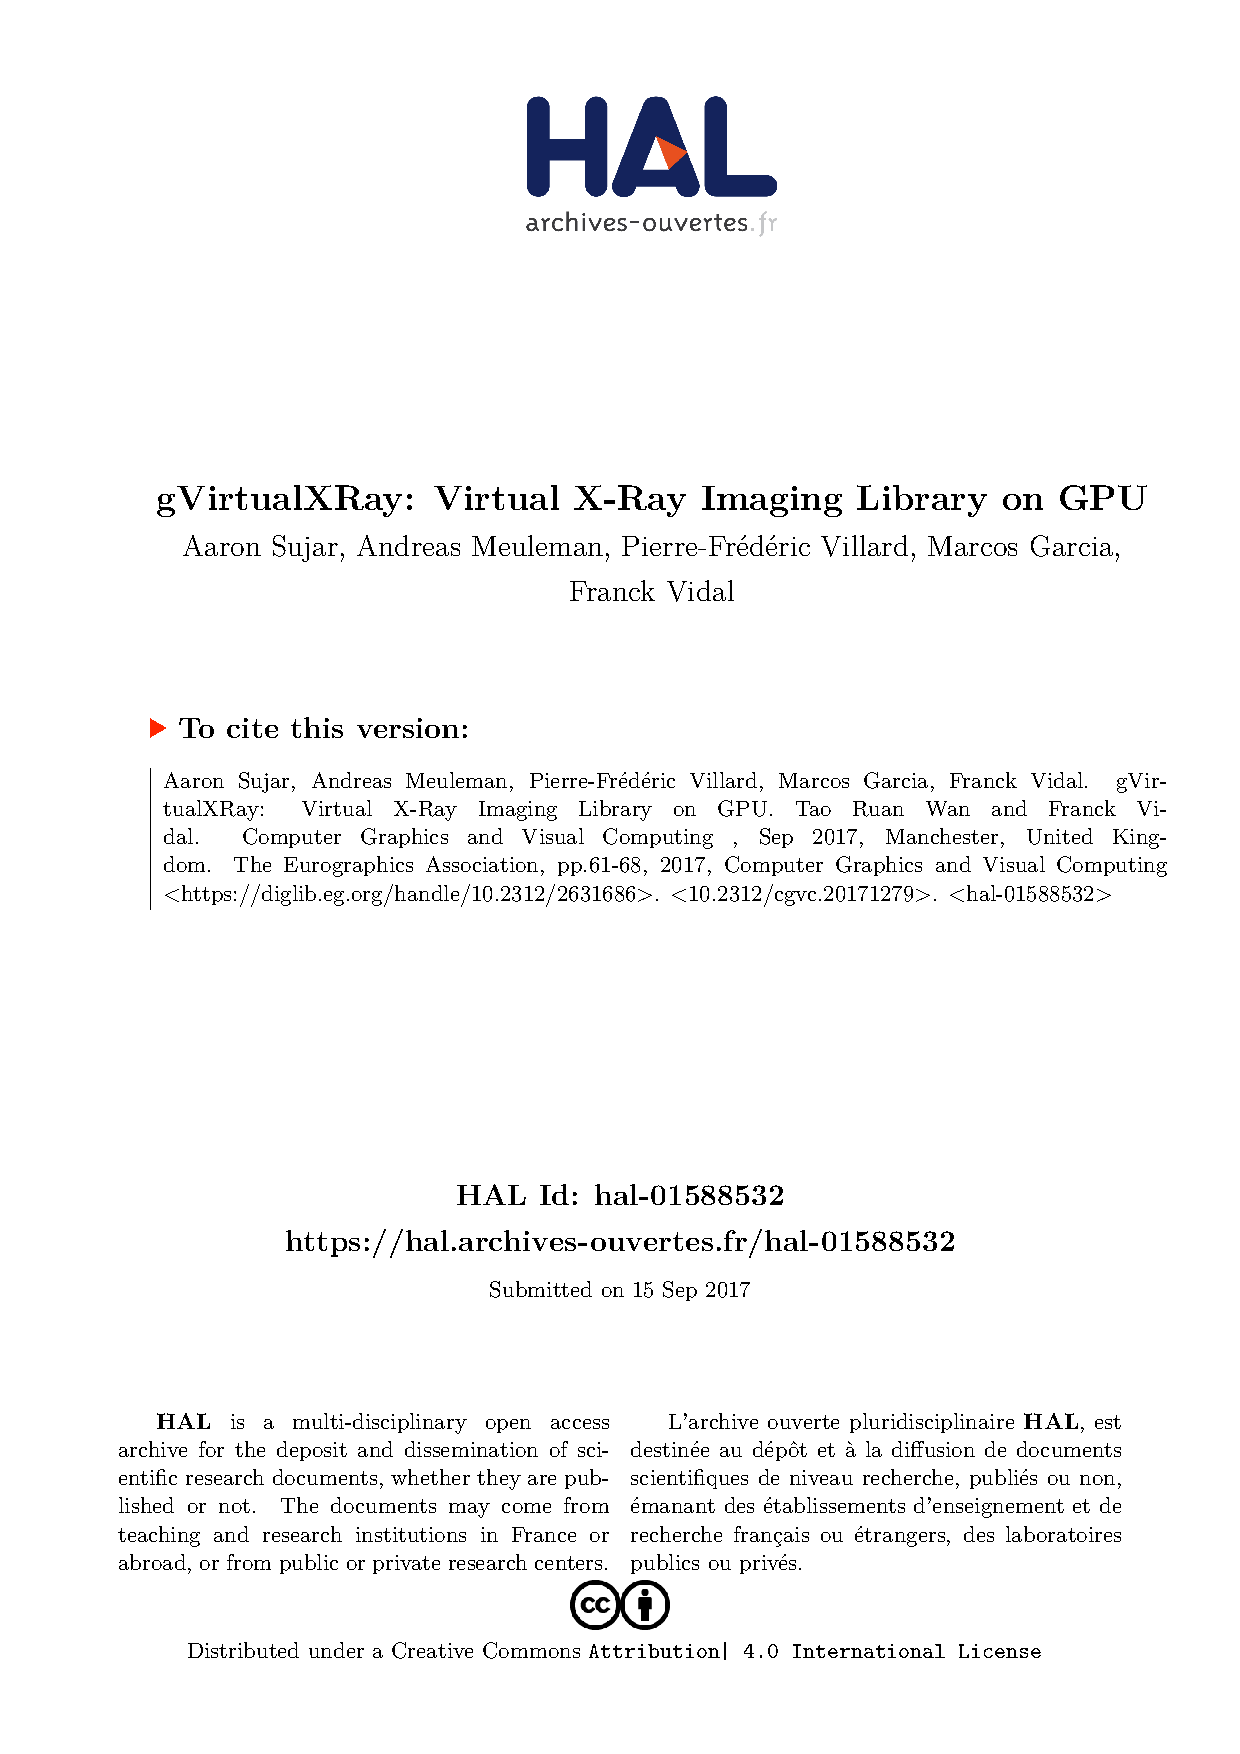
\includepdf[pages=1,scale=0.8,
pagecommand={\section{gVirtualXRay: Virtual X-Ray Imaging Library on GPU}
\label{anexo:cguk}},linktodoc=true]{PDFs/cguk}
\includepdf[pages=2-,scale=1,pagecommand={},linktodoc=true]{PDFs/cguk}


\includepdf[pages=1,scale=0.8,
pagecommand={\section{Real-time animation of human characters’ anatomy}
\label{anexo:cag}},linktodoc=true]{PDFs/cag}
\includepdf[pages=2-,scale=0.9,pagecommand={},linktodoc=true]{PDFs/cag}


\includepdf[pages=1,scale=0.8,
pagecommand={\section{Interactive learning environment for diagnostic radiographywith real-time X-ray simulation and patient positioning}
\label{anexo:xray}},linktodoc=true]{PDFs/XRAY}
\includepdf[pages=2-,scale=1,pagecommand={},linktodoc=true]{PDFs/XRAY}






%\appendix
%\include{appendix}
\cleardoublepage
% Como incorporar como un capitulo mas en el indice de la bibliografia
\addcontentsline{toc}{chapter}{Bibliografía}
\bibliography{bibliography}
\bibliographystyle{alpha}
\end{document}
